%\documentclass[aps,pra,reprint,longbibliography]{revtex4-1}
\documentclass[twocolumn]{article}

\usepackage{geometry}
\geometry{textwidth = 18cm,textheight = 24cm}

%\usepackage{multicol}
\usepackage{caption}

\usepackage{graphicx}
\usepackage{amsmath}
\usepackage{float}
%\usepackage{amssymb}
\usepackage{textcomp}
%\usepackage{lmodern}
\newenvironment{figure_alt}
  {\par\medskip\noindent\minipage{\linewidth}}
  {\endminipage\par\medskip}

\begin{document}
	
	%-------------------- begin header -------------------%
	\centerline{\LARGE Optoelectronic Intelligence}%Light in neural systems%Intelligent optoelectronic systems
	\vspace{0.75em}
	\centerline{\Large Jeffrey M. Shainline}
	%\vspace{0.75em}
	%\centerline{\large National Institute of Standards and Technology}
	\vspace{0.5em}
	\centerline{\large NIST, Boulder, CO, 80305}
	\vspace{0.5em}
	\centerline{\large \today}
	%-------------------- end header ---------------------%

	
%\author{Jeffrey M. Shainline\\National Institute of Standards and Technology, 325 Broadway, Boulder, CO, 80305}
%\affiliation{National Institute of Standards and Technology, 325 Broadway, Boulder, CO, 80305}		
	
%\date{\today}
	
\begin{abstract}

\end{abstract}

%\begin{multicols}{2}

\section{\label{sec:introduction}Introduction}
Light is excellent for communication. Fiber optic links carry vast quantities of information across continents and between data centers. An important question in modern computing is: what is the shortest distance over which photonic communication will displace electronic interconnects? Optical links between racks in data centers are becoming common \cite{}. Major companies are investing seriously in photonics in the package. Monolithic optical links between processor and memory fabricated in a 45-nm CMOS node with no in-line changes have been demonstrated \cite{suwa2015}. A primary challenge affecting further chip-scale electronic-photonic integration is the continued difficulty of achieving a light source implemented on silicon that is robust, efficient, and economical.

In parallel with the hardware considerations affecting optoelectronic integration are questions related to architecture. A prominent theme emerging since clock speed leveled off in 2003 \cite{} is parallelism. Computation is increasingly distributed among more processor cores. Many-core architectures continue to expand into on-chip networks, in some cases resulting in highly distributed, brain-inspired systems \cite{}. As compute grows more distributed, communication across interconnection networks becomes a bottleneck. The demand for energy efficient communication bandwidth has been a major driver of on-chip photonics.

The major drivers for brain-inspired computers fall on a spectrum: energy and algorithmic efficiency for deployable applications reside on one side of the spectrum, and artificial general intelligence (AGI) resides on the other. Knowledge gained from neuroscience informs us that systems with general intelligence will benefit from very large numbers of computational elements as well as extreme communication between them. It is our perspective that hardware incorporating light for communication between electronic computational elements combined with an architecture of distributed optoelectronic spiking neurons will provide tremendous potential for AGI. Considerations pertinent to the realization of such a technology are the subject of this article.

\section{\label{sec:neuroFractalsAndVLSI}Neuroscience, fractal geometry, and very-large-scale integration}
To guide the design of hardware for AGI, we must simultaneously consider the principles of neural information and very-large-scale integration (VLSI). Both lead to fractal scaling.

Information processing in neural systems employs local clusters of neurons to represent specific features, and the information from these clusters must be shared with other regions of the network to form a multifaceted representation of a complex stimulus. The dynamical patterns of activity that accomplish this information integration are neuronal avalanches, cascades of spiking activity across local, regional, and global partitions of the network. We denote by $s$ the number neurons involved in a neuronal avalanche. Brain activity across many species, brain regions, and contexts shows the probability of observing an avalanche of size $s$ follows a power law: $P(s)\sim s^{-\alpha}$. Systems with a power-law distribution of neuronal avalanches demonstrate self-organized criticality \cite{}, which maximizes the dynamic range of the system \cite{}. Such a power-law dependence has the important property that the ratio of number of events of size $qs$ to the number of events of size $s$ is simply $q^{-\alpha}$, independent of $s$. For this reason, such a distribution is referred to as ``scale-free'', and is self-similar, or fractal, across spatial and temporal scales. 

Fractal properties of neural systems are crucial to their operation. Fractal systems can continue to scale, with dynamics constrained only by the physical hardware and spatial extent of the system rather than by the ability to communicate across the architecture \cite{plth2007}. Such scale-free systems can efficiently integrate information from local clusters to vast networks, while enabling correlations across wide regions of space and long periods of time. 

Achieving the necessary communication for scale-free systems across space and time places severe demands on hardware. The physical requirements for supporting neuronal avalanches across a broad range of scales can be understood from the perspective of Rentian scaling, first explored in the context of VLSI microelectronic circuits \cite{}. Rentian analysis tracks the relationship between the number of nodes within a volume of space and the number of connections emanating from that volume for partitions of the network from a single node to the network as a whole. It has been observed empirically that a wide variety of systems from electronic processors to biological neural networks obey a relationship of the form $e_i\sim n_i^{\beta}$, where $e_i$ is the number of edges emanating from the $i$th hierarchical partition of the network, $n_i$ is the number of nodes confined within that partition, and $\beta$ is referred to as the Rent exponent. Again, a scale-free relation is found. To best achieve Rentian scaling across very large systems, and thereby enable large neuronal avalanches, optical communication infrastructure is necessary. 

%These considerations of network structure reveal important considerations for the design of neural hardware that form the foundation of our argument that light should be used for communication in artificial neural systems. 

The dynamical attributes of the network that give rise to neuronal activity across spatial and temporal scales must also be considered. The synaptic connections between neurons play a crucial role in enabling complex, dynamic activity. Short-term synaptic plasticity enables synapses to rapidly adapt in response to network activity, essentially resulting in temporal filtering of afferent spike trains \cite{abre2004}. Learning in the presence of a continually changing environment while maintaining long-term memories is achieved through spike-timing-dependent plasticity (STDP) \cite{somi2000} and metaplasticity \cite{ab2008}. Dendritic processing, wherein the dendritic arbor performs intermediate, nonlinear transformations between synapses and the soma, enables utilization of timing information \cite{vagu2005}, detection of sequences of activity \cite{haah2015}, and in conjunction with inhibitory interneurons enables specific inputs to be silenced or augmented at specific times \cite{bu2006}. A combination of excitatory and inhibitory neurons with complex plasticity mechanisms and dendritic processing allows a given structural network to implement a wide variety of dynamical functions, and allows efficient access to and integration of information across broad spatial and temporal scales. Dynamical electronic neurons and synapses can rapidly adapt the vast structural network enabled by photonic communication into myriad functional networks. 

%These consideration of network and device dynamics form the foundation of our argument that electrical circuits should be used for computation in artificial neural systems. 

This brief foray brings a few key messages relevant to the design of artificial neural hardware. Diverse activity across spatial and temporal scales requires a vast structural interconnection network with communication across spatial scales, as captured by Rentian scaling. We conjecture that light is most capable of achieving communication in complex neural systems, from the scale of local clusters to the entirety of an AGI. But neural activity also requires components adapting at various frequencies to enable myriad functional networks, as demonstrated by neuronal avalanches with activity at various frequencies, enabled by complex, adaptive synapses and dendrites. Such complex, adaptive activity is much better suited to the domain of electronic circuitry. Based on these consideration, we expect a hardware platform capable of AGI to combine the strengths of photonic communication with electronic computation to integrate information in neuronal avalanches from small, local clusters on a silicon wafer to the light-cone-limited region of space across which light can travel in a network oscillation cycle. 

%Based on these considerations, we expect a hardware platform capable of AGI to display at least six traits. Intelligent neural hardware will incorporate 1) plasticity mechanisms that allow rapid incorporation of new information as well as long-term memory retention \cite{fudr2005,fuab2007} while adapting to maximize dynamic range in response to stimulus \cite{shki2006}; 2) dendritic nonlinearities that work in conjunction with inhibition to enable attention to be directed to certain stimuli \cite{bu2006} as well as enable sequence detection \cite{haah2015} and temporal coding \cite{}; 3) spiking neuronal dynamics based on relaxation oscillators, as this form of computation and communication appears uniquely suited for information integration across space and time \cite{bu2006}; 4) massive connectivity to enable short path lengths across large networks \cite{sp2010}; 5) the ability to efficiently use space from the scale of a single synapse up to systems limited by light-speed communication, and the ability to efficiently use time with network oscillations across a wide range of frequencies; and 6) energy consumption and power density low enough to enable scaling to systems of this size.

%Regarding the fabrication of large systems, we assume success developing AGI is most likely if the infrastructure developed for digital computing with silicon electronics can be utilized. This leads us to at least five traits that hardware must display if extreme scalability is to be achieved. Fabrication is most likely to succeed if: 1) it is based on lithography on silicon wafers; 2) features are large enough to be patterned with 193 nm light sources ($> 50 nm$ is best); 3) no materials crucial to the system are rare, volatile, or incompatible with conventional processing; 4) multi-wafer modules should be achievable, as human-scale intelligence is not likely to be achieved on a single wafer; and 5) for very large systems with photonic connectivity, the ability to leverage fiber optic technology will likely be highly advantageous.

\section{\label{sec:synapsesDendritesAndNeurons}Optoelectronic synapses, dendrites, and neurons}
The device factors mentioned above are not quirks of the biological world, but rather are some of the reasons brain computation is so complex and efficient. Short-term plasticity produces information about spike train rising and falling edges and guards against runaway activity. STDP strengthens correlations between neurons that fire constructively and dampens connections that waste energy. These mechanisms have been shown to adapt random structural networks into complex functional networks with small-world architecture and neuronal avalanches indicating maximal dynamic range due to criticality. Dendritic processing in conjunction with inhibitory interneurons makes efficient use of the complex spatial network by dynamically activating a wide range of functional networks. To achieve these myriad computational functions, optical interactions are inadequate. The complexity of electronic circuits is required. 

We envision optoelectronic hardware with communication along photonic axons, and computation performed in electronic synapses, dendrites, and neurons. We make two more choices to specify the platform. Detectors must respond to single photons for maximal energy efficiency. Superconducting-nanowire single-photon detectors (SNSPDs) are the clear choice for this application, with very low dark counts, near-zero static power dissipation, and scalable integration \cite{shbu2017b}. An SNSPD is simply a current-biased strip of superconducting wire roughly 100\,nm in width and 5\,nm in thickness. SNSPD operation is summarized as follows. In the steady state, the current bias flows straight to ground, and upon detection of a photon, a small section of the wire is driven from the superconducting phase to the normal-metal phase, resulting in a transient resistance of a few kilo-ohms for a few hundred picoseconds. This resistance produces a transient current bias a load. 

In addition to the choice of SNSPDs as the detectors in the system, we must also identify the most promising light source, which must be fabricated across wafers by the millions for economical, brain-scale systems. Because our choice of detectors dictates cryogenic operation, silicon light sources operating at 4\,K are an option \cite{da1989,shxu2007}. This neural system may be one of the few applications where silicon light sources are appropriate and sufficient. The light sources we have in mind are silicon LEDs, employing luminescence from defect-based dipole emitters \cite{buch2017}. From the perspective of VLSI, achievement of a silicon light source of sufficient performance would be the greatest contribution to the success of this technology.

To achieve complex neural circuits, we must combine light sources, detectors, and various other circuit elements. We have demonstrated waveguide coupling of light from these micron-scale light sources to integrated SNSPDs on a silicon photonic chip \cite{buch2017}. The detectors can be engineered in circuits with Josephson junctions (JJs) and superconducting loops coupled through mutual inductors to achieve the complex circuit functions we need for neural information processing. The current bias across a single JJ establishes the synaptic weight. This current bias can be modified through various photonic and electronic means based on network activity. Inhibition is straightforward with opposing mutual inductors. Dendritic and neuronal nonlinearities are a natural consequence of phase slips across JJs driven above their critical current, and the extreme nonlinearity of the superconducting phase transition playing a leading role, both for the detection of light at synapses and for the production of sufficient voltage to generate light during neuronal firing events. Due to the prominent role of superconducting current storage loops, we refer to these as loop neurons. In the operation of loop neurons, a single photon triggers a synaptic event, and STDP is induced by two photons\textemdash one from each neuron associated with the synapse. %Such hardware appears promising to achieve extreme communication across vast networks while maintaining very low power density, and reasonable system power consumption.

%We call attention to one aspect of this approach to photonic synapses that differs from other approaches being pursued in the community. In optoelectronic hardware leveraging light for communication, there are two general approaches to change the synaptic weight between two neurons: 1) in the photonic domain with variable attenuation of an optical signal; or 2) in the electronic domain with a variable electronic response upon detection of an optical pulse. This choice has several important ramifications for hardware and information processing. Regarding information processing, it is usually assumed that neural communication is digital: the presence or absence of an action potential is a binary one or zero, and the amplitude of the action potential does not encode information. When adjusting the synaptic weight in the photonic domain, this is not the case. The number of photons reaching a neuron through a synaptic connection becomes an analog variable, and it is subject to shot noise, in addition to any noise mechanisms present in the detector. The signal-to-noise ratio of shot noise improves with $\sqrt(N_{\mathrm{ph}})$, where in this case $N_{\mathrm{ph}}$ is the average number of photons, so establishing weights in the photonic domain introduces an energy/noise tradeoff. Setting weights in the photonic domain also has the disadvantage that photons are discarded by attenuation at weak synaptic weights. Thus, by setting synaptic weights in the photonic domain, we place a burden on light sources to produce large numbers of photons to minimize shot noise, and we discard photons when they are attenuated at weak synapses. In this mode of operation, light is used for communication, but it is also used for the important computational operation of applying the synaptic weight.

%By contrast, if we establish synaptic weights in the electronic domain (as is accomplished with a bias current across a JJ in a loop neurons), light is used exclusively for communication, and communication remains entirely digital. In this case, the detector and associated electronics must be able to achieve a variable synaptic response to photonic pulses based on the configuration of the electronic aspects of the circuit. In this case, we expect that a neuron will send, on average, $N_{\mathrm{ph}}$ photons to each of its downstream synaptic connections. Due to shot noise, each downstream connection will receive $N_{\mathrm{ph}}\pm\sqrt{N_{\mathrm{ph}}}$ photons, and the detector circuit must be configured to implement a synaptic response if a threshold of $N_{\mathrm{th}}$ or more photons is detected. After detection, the electronic response must vary depending on the synaptic weight, independently of the precise number of photons detected. It is in this electronic response that the signal becomes analog again. Whereas setting the synaptic weights in the photonic domain places a larger burden on light sources, setting the synaptic weights in the electronic domain places a larger burden on detector circuits. These reconfigurable bias currents or voltages represent the synaptic weights, and the task of a neuron's light source is simply to provide a roughly constant number of photons to each of its downstream synaptic connections. For energy efficiency, the number of photons necessary to evoke a synaptic response from the detector ($N_{\mathrm{th}}$) should be made as low as possible to make the job of the light source as easy as possible. $N_{\mathrm{th}}$ cannot be made lower than one, as the electromagnetic field is quantized into integer numbers of photons, and it is at this limit that loop neurons aspire to operate. It is our opinion that establishing synaptic weights in the electronic domain is necessary to enable the complex synaptic, dendritic, and neuronal behaviors that make neural information processing powerful. 

%Having made the choice to communicate with light, one must devise a means to perform the necessary device functions of neural systems. One such function is establishment of a synaptic weight. Synaptic weights are the primary form of long-term memory in neural systems, and they change the strength of connections between neurons \cite{daab2001,geki2002}. In optoelectronic hardware leveraging light for communication, there are two general approaches to change the synaptic weight between two neurons: 1) in the photonic domain with variable attenuation of an optical signal; or 2) in the electronic domain with a variable electronic response upon detection of an optical pulse. This choice has several important ramifications for hardware and information processing. Regarding information processing, it is usually assumed that neural communication is digital: the presence or absence of an action potential is a binary one or zero, and the amplitude of the action potential does not encode information. When adjusting the synaptic weight in the photonic domain, this is not the case. The number of photons reaching a neuron through a synaptic connection becomes an analog variable, and it is subject to shot noise, in addition to any noise mechanisms present in the detector. The signal-to-noise ratio of shot noise improves with $\sqrt(N_{\mathrm{ph}})$, where in this case $N_{\mathrm{ph}}$ is the average number of photons, so establishing weights in the photonic domain introduces an energy/noise tradeoff. Setting weights in the photonic domain also has the disadvantage that photons are discarded by attenuation at weak synaptic weights. Thus, by setting synaptic weights in the photonic domain, we place a burden on light sources to produce large numbers of photons to minimize shot noise, and we discard photons when they are attenuated at weak synapses. In this mode of operation, light is used for communication, but it is also used for the important computational operation of applying the synaptic weight.

%By contrast, if we establish synaptic weights in the electronic domain, light is used exclusively for communication, and communication remains entirely digital. The presence of an optical signal can be used to represent an all-or-none communication event. In this case, the detector and associated electronics must be able to achieve a variable synaptic response to identical photonic pulses based on the configuration of the electronic aspects of the circuits. In this case, we expect that a neuron will send, on average, $N_{\mathrm{ph}}$ photons to each of its downstream synaptic connections. Due to shot noise, each downstream connection will receive $N_{\mathrm{ph}}\pm\sqrt{N_{\mathrm{ph}}}$ photons, and the detector circuit must be configured to implement a synaptic response if a threshold of $N_{\mathrm{th}}$ photons is detected. After detection, the electronic response must vary depending on the synaptic weight, independently of the precise number of photons detected. It is in this electronic response that the signal becomes analog again. Whereas setting the synaptic weights in the photonic domain places a larger burden on light sources, setting the synaptic weights in the electronic domain places a larger burden on detector circuits. One must achieve a detector circuit that converts light pulses to electrical current or voltage, and the amount of electrical signal must be largely independent of the number of photons in the pulse, depending instead on reconfigurable electrical properties of the circuit, such as bias currents or voltages. These reconfigurable bias currents or voltages then represent the synaptic weights, and the task of a neuron's light source is simply to provide a roughly constant number of photons to each of its downstream synaptic connections. For energy efficiency, the number of photons necessary to evoke a synaptic response from the detector ($N_{\mathrm{th}}$) should be made as low as possible to make the job of the light source as easy as possible. $N_{\mathrm{th}}$ cannot be made lower than one, as the electromagnetic field is quantized into integer numbers of photons. 

%To reach the energy efficiency limit of $N_{\mathrm{th}}=1$ while setting the synaptic weight in the electronic domain, we proposed utilizing optoelectronic circuits combining superconducting-nanowire single-photon detectors (SPDs) \cite{mave2013} in conjunction with Josephson junctions (JJs) \cite{ka1999} as synaptic receivers \cite{sh2018}. We refer to these circuits as loop neurons, and they have several desirable properties. First, they have very near zero dark counts, and their response is nearly identical whether they receive one or more than one photon within a short time window, so the quantity $N_{\mathrm{th}}$ can be made as low as physically possible. Second, because the circuit is not attempting to resolve the number of photons present in a pulse, shot noise on the photonic communication signals does not propagate beyond the synapse. Instead, the average number of photons arriving at a synapse simply must be high enough that the probability of a synapse receiving zero photons becomes tolerably small ($N_{\mathrm{ph}} = 5$ gives a 1\% chance of receiving zero photons). Third, the synaptic weight in this circuit is set by a current bias across the Josephson junction, which has nearly zero effect on the behavior of the SPD, and can be straightforwardly adjusted to achieve a wide range of synaptic weights. The effect of this current bias is to change how much current gets added to the neurons integrated signal when a photon is detected. Fourth, in addition to the energy benefits derived from signaling with order one photon, superconducting detectors dissipate zero power in the steady state. Amidst these benefits lies a challenge: to realize these synapses, one must integrate SPDs with JJs in a scalable hardware platform. It is our perspective that such hardware will bring significant capabilities for AGI, in part due to the efficient, low-noise operation of these single-photon optoelectronic synapses.

%Following the question of whether synaptic weights are set in the photonic or electronic domain lies the question of how the synaptic weights are modified. Synaptic weight modification is a primary means of signal processing and learning in neural systems. In machine learning, synaptic weights are often trained through backpropagation wherein the output of a network is compared to a desired output, and synaptic weights are updated to minimize a cost function. For AGI systems interacting with complex, dynamic environments, cost functions associated with all inputs to the network generally cannot be defined, so supervised learning algorithms such as backpropagation are conceptually poorly matched to the learning requirements. Further, brain-scale systems can be expected to employ $10^{14}$ synapses connected in highly recurrent graphs, so scalable learning must be accomplished by mechanisms local to the synapses and cannot afford to rely on an external supervisor making contact to each synapse independently. 

%In STDP, the timing between pulses from the pre-synaptic neuron and post-synaptic neuron change the strength of the synaptic connection \cite{somi2000}. When designing optoelectronic synapses for AGI systems, the ability to perform both strengthening and weakening depending on the order of pre- and post-synaptic activity at each synapse is vital. For applications in deep learning, interferometric networks have been proposed to leverage light for matrix-vector multiplication \cite{}. In such an implementation, the phases applied throughout the network determine the synaptic weights, but changing a single phase changes multiple synaptic weights, in general. Thus, there appears to be no way to utilize this approach to achieving synaptic weights to implement STDP. Another approach to setting synaptic weights in the photonic domain utilizes variable attenuation of a phase-change material \cite{}. In this case, the absorption of photons can modify the atomic configuration of the material, providing a means by which the presence of optical signals can reduce material absorption and thereby modify the synaptic weight. It has been shown that this technique can be used to achieve Hebbian learning wherein the simultaneous arrival of photons from pre-synaptic and post-synaptic neurons reduces attenuation and increases synaptic weight. The materials demonstrated to date require billions of photons for this operation, so energy efficiency is a concern for scaling. Additionally, while Hebbian strengthening is straightforward with this approach, it may not be possible to decipher the order of arrival of the pulses, so anti-Hebbian weakening and full STDP may not be possible. In the context of loop neurons, STDP can be straightforwardly achieved based on correlated detection events of a single photon from the pre-synaptic neuron and a single photon from the post synaptic neuron \cite{sh2018}. Hebbian or anti-Hebbian detection events increase or decrease the current bias across the synaptic JJ, thereby achieving STDP at the lowest possible light level of a single photon for each step of the update process. 

%STDP is an important mechanism that enables learning based on local activity of two neurons. In addition to this mechanism that modifies synaptic memory, it has been found that the ability to change not only synaptic weights, but also the rate at which synaptic weights are modified is an important capability to enable simultaneous acquisition of new knowledge and long-term memory retention \cite{}. Mechanisms that change the rate of synaptic weight update are referred to as metaplasticity \cite{ab2008}. Incorporating metaplasticity into artificial cognitive systems is necessary to enable the system to maintain a robust representation of past experiences while learning from a constantly changing environment. In optoelectronic hardware, the device-level operation that accomplishes metaplasticty will depend on how one has chosen to establish the synaptic weight in the first place. In the case of loop neurons the amount a synaptic weight is incremented during an STDP event depends on a bias current across a JJ, just as the synaptic weight itself depends on a bias current across a JJ. Metaplasticity is accomplished by modifying this synaptic update bias current, again based on detection of photons generated during neuronal firing events indicating the level of network activity. Like other operations in loop neurons, metaplastic update can be achieved with SPDs working in conjunction with JJs: photon detection events generate electrical current that changes the state of the synapse to make STDP more or less substantial. 

%In addition to STDP and metaplasticity, which affect synaptic weights and their rates of change over time scales long to relative to the time between pulses in a train (inter-spike interval), short-term plasticity is a crucial aspect of the behavior of a synapse that affects synaptic behavior on a time scale of the inter-spike interval. Short-term plasticity serves to filter input pulse trains. Short-pass, long-pass, and band-pass behavior have all been observed in biological neural systems. Short-pass filtering of spike trains causes the synapse to fire only at the beginning of an afferent spike train, while long-pass filtering leads to a synapse becoming active only after an multiple pulses of a train have been received. Band pass filtering ensures that a synapse does not respond to the first few pulses in a train (rising edge of the signal), but becomes responsive during a number of pulses in the middle of a sequence, before saturating and again going quiet during the final pulses of a train (falling edge of the signal). These rapid modifications of synaptic behavior are crucial to provide a neuron with a rich picture of the temporal activity input to its synapses, yet such complex behavior is difficult to achieve for many methods of establishing synaptic weights in photonic systems. It is our perspective that achieving STDP, metaplasticity, short-term plasticity, and other adaptive synaptic properties is significantly facilitated if electronic circuits perform the adaptation, affecting the response of the electrical circuit to the detection of photonic communication events. In loop neurons, all these functions appear straightforward in simulations of superconducting circuits of modest complexity. Similar functions may be possible using CMOS devices in conjunction with semiconductor photodetectors. Whether at room-temperature or 4\,K, optoelectronic synapses wherein electronic circuits receive photonic communication events and adapt synaptic behavior based on these optical signals are necessary for enabling complexity in intelligent optoelectronic neural systems. Light is excellent for communication, but electronics excel at computation.

%While much computation in neurons occurs in synapses, the nonlinear response of the neuron itself is the primary computation performed on the inputs from all the neuron's synapses. In spiking neurons, this nonlinearity manifests as the production of a pulse when the integrated signal reaches threshold. Spiking neurons perform the a rate-in/rate-out transfer function. The leak rate of the integrated signal determines the turn on input rate, and the refractory period (reset time) determines the roll-over point of this transfer function. Thus, in addition to the nonlinearity associated with reaching threshold and producing a spike, neurons exhibit a nonlinear spike rate transfer function. 

%As emphasized above in the discussion of neuronal avalanches, neural systems display activity with structure across a wide range of temporal scales. Activity at lower frequencies will generally encompass information from a larger region of the network, while activities at higher frequencies will generally integrate information locally to build consensus amongst a smaller population of the network. Achieving a short refractory period enables fast oscillations, and is therefore important to achieving rapid interpretation of new stimulus. Photonic systems such as excitable lasers can achieve extremely fast reset times, and have thus received significant attention as relaxation oscillators for spiking neural systems \cite{dukr1999,prsh2017}. However, it remains important for a neuron to maintain information regarding stimulus received in the past related to low-frequency, network-wide activity, so the leak rate of the neuron should be made as long as possible. If one attempts to utilize an optical cavity as an integrator of photons received from upstream connections, the leak rate will be limited by the photon lifetime in the cavity, $\tau = Q/\omega_0$, where $Q$ is the cavity quality factor, and $\omega_0$ is the angular frequency of electromagnetic wave. $Q$ of $10^{6}$ is difficult to achieve in integrated laser systems, and even with this high-$Q$ we find $\tau =$\,1\,ns for photons at 1550\,nm, indicating that integrating photonic signals in the optical domain makes it very difficult for a neuron to retain information relevant to lower-frequency, larger-area network activity. The response of such a neuron is independent of anything that happened in the network longer ago than $\tau$, and the neuron can not identify correlations between local, rapid activity, and broader, slower activity.

%Like the case of synaptic computations and plasticity, we reach the conclusion that the neuronal computation of signal integration is best performed in the electronic domain. This operation requires that a photodetector operate in conjunction with an electronic circuit to transduce photon detection events to stored electrical charge or current. If semiconducting circuit infrastructure is employed, this stored electrical signal will likely be charge on a capacitor resulting in voltage, and when the accumulated voltage reaches a given threshold, the electrical circuit must generate (or modulate) light, presumably via a semiconductor diode. If superconducting circuit infrastructure is employed, the stored electrical signal is supercurrent circulating in a loop, and the threshold is set by the critical current of a JJ. This superconducting implementation has the advantage that the signal can be maintained indefinitely (provided superconductivity is maintained), so the integration time $\tau$ can be chosen to be as long as theoretical analysis deems appropriate, and can be implemented in hardware with the $L/r$ time constant of the integration loop. The integration time of the neuron is completely decoupled from the threshold of the neuron as well as all other aspects of the circuit. The primary challenge of this superconducting loop neuron design is to achieve the voltage necessary to produce light from a semiconductor diode when threshold is reached \cite{sh2018d}. Fortunately, significant experimental progress has recently been made demonstrating the feasibility and efficiency of such an operation \cite{mcve2018}.

%In addition to these synaptic and neuronal computations, the significance of intermediate dendritic nonlinear processing is increasingly being emphasized by the neuroscience community \cite{stsp2015}. 

%Dendrites:
%\begin{itemize}
%\item Dendritic nonlinearities can in principle be in either photonic of electronic domain. Photonic domain, nonlinearities require quite a bit of power (saturable absorbers, frequency conversion)
%\end{itemize}
%
%Neurons:
%\begin{itemize}
%\item Spiking neural dynamics requires that, upon reaching threshold, pulses of light must be produced
%\item this has led some to propose excitable lasers as neurons. light detected by photodetector, fan-in, time constants, power required
%\item integration should be performed in the electronic domain, and upon reaching an electronic threshold, a voltage pulse can be produced to either generate light or modulate an externally provided cw light stream
%\item for communication across a branching network of passive photonic waveguides, coherence of light source is not required
%\item choice of light source is crucial (on or off chip, material, wdm or not, wavelength)
%\end{itemize}
%
%discussion of frequency (each neuron cannot have its own frequency due to practical limitations, selection and routing of neuronal communication signals cannot be achieved by frequency alone)


\section{\label{sec:communication}Communication with guided light}
The central premise of our work is that photonic signals are superior to electronic signals for communication across large-scale neural systems. To explain why we place this conjecture at the center of hardware development, we briefly summarize the physical limitations of electrical interconnection networks \cite{hepa2012}. It is impracticable in silicon electronics for a single device to source current to many other devices, so in practice a shared communication network is employed \cite{}. In contemporary computing, switched media networks are used for this purpose. Each device must then only communicate to the nearest switch in the network. The interconnect network determines a valid route for the information to traverse across the network, and the switches are configured accordingly. Because the communication infrastructure is shared, devices must request access to the switch network to transmit messages. When multiple devices request access simultaneously, arbitration must be performed, wherein devices are queued and sequentially granted access to the switch network. This approach to communication between electronic devices leverages the speed of electronic circuits to compensate for the difficulties in communication. The limitations are reached when many devices need to communicate with many other devices with a high frequency of communication events. Unfortunately, this is exactly the situation encountered in neural information processing. During a neuronal avalanche, many neurons may need to communicate simultaneously across the network. As more neurons, each with many synapses, are added to the network, the average frequency of neuronal firing events must decrease due to the limitations of the interconnection network to handle communication requests, and large neuronal avalanches integrating information across the network cannot be supported by the communication infrastructure. %For electronic systems with a few hundred thousand neurons, average event rates in the kilohertz range can be maintained \cite{}. Systems with a few hundred million neurons will likely be limited to operation at 10 Hz or below \cite{}.

%In a switched media network, devices communicate with one another by sending packets of information. The packet contains routing information (the address of the recipient) as well as the data to be communicated.

%\subsection{\label{sec:electricalInterconnectionNetworks}Electrical interconnection networks}
%When using silicon electronics, information is represented by voltages. A voltage is achieved physically by accumulating charge on a capacitor. For one device to communicate information to another device, it must provide charge in the form of electrical current. This current must charge up the capacitors representing information at the target device as well as the capacitance of the wire over which the charge is transferred. There are fundamental and practical limits to how small the capacitance of the devices and wires can be \cite{}. As a rule of thumb, a wire in a CMOS process adds 200\,aF/\textmu m, so parasitic wire capacitance dominates when devices are separated by even a few microns. It becomes impracticable for a single device to source current to many other devices, so in practice a single transistor rarely drives more than four other transistors (fanout of four). For many applications, it is crucial for each device to be able to send information to many more than four destinations. Because all the devices requiring communication with one another cannot be directly wired to each other, a shared communication network is employed. In contemporary computing, switched media networks are used for this purpose. Each device must then only communicate to the nearest switch in the network. In a switched media network, devices communicate with one another by sending packets of information. The packet contains routing information (the address of the recipient) as well as the data to be communicated. The interconnect network determines a valid route for the information traverse across the network (referred to as routing), and the switches are configured accordingly to achieve that physical route of information transfer. 

%Because the communication infrastructure is shared devices must request access to the switch network to transmit messages. Multiple devices may request access simultaneously, in which case arbitration must be performed. Arbitration refers to the process of granting devices access to the switch network, and in general a packet will experience some delay while it waits in a queue to be granted access to the shared communication infrastructure. This process of serializing communication across a common interconnection network is referred to as time multiplexing. This approach to communication between electronic devices leverages the speed of electronic circuits to compensate for the difficulties in communication. For many applications this is adequate. The limitations are reached when many devices need to communicate with many other devices with a high frequency of communication events. Unfortunately, this is exactly the situation encountered in neural information processing. When implementing neural information processing with electronic communication infrastructure, neuron pulses are represented as packets of data called events. Some of the data in a packet representing an event must contain the addresses of the synapses to which the event should be communicated. This type of neural information processing is therefore referred to as address-event representation. One consequence of this approach is that as the size of the system grows, more information in each communication event must be allocated to specifying destinations. This leads to increased burden on memory and processors. But the more severe challenge is introduced by the connectivity/speed trade-off. As more neurons, each with many synapses, are added to the network, the average frequency of neuronal firing events must decrease due to the limitations of the interconnection network to handle communication requests. For electronic systems with a few hundred thousand neurons, average event rates in the kilohertz range can be maintained \cite{}. Systems with a few hundred million neurons will likely be limited to operation at 10 Hz or below \cite{}. 

%\subsection{\label{sec:photonicInterconnectionNetworks}Photonic interconnection networks}
The requirement of utilizing a shared communication infrastructure results from the physics of electrons. Because electrons interact with each other due to their charge, they can be used to establish a voltage on a capacitor, which is useful for computing. But the charge-based interaction is also what makes it difficult to source sufficient current to directly communicate between many devices. The physics of light is complimentary to that of electrons. Photons, being uncharged bosons, interact with one another only through quantum interference, such as the Hong-Ou-Mandel effect. Light-matter interaction is generally weak, especially at low light levels. Thus, photons can co-propagate on waveguides independently of one another without wiring capacitance. This enables a pulse of photons to fan out to many destinations without a charging penalty due to wiring. This is not to say photonic communication can address an arbitrarily large number of recipients without consequence. For each new recipient, the number of photons in the initial pulse must increase, and as destinations get further away, more energy is dissipated to propagation loss. These realities notwithstanding, it appears feasible for devices communicating with photons to make direct, physical, point-to-point connections to many thousands of destinations, thereby eliminating the need for the shared communication infrastructure that is the primary impediment to achieving AGI with electrical interconnections.

Having made this claim, the burden is upon us to provide evidence of the feasibility of photonic communication in large-scale neural systems. Much like electrical interconnection networks utilize different technologies at the scales of chips versus data centers, photonic interconnection technologies must enable communication from the scale of an on-chip network to a many-wafer system the size of a data center. Further, the specific architectures suitable for neural information processing require that neurons be capable of communicating seamlessly across all scales of this network hierarchy. At the outset, the large wavelength of light relative to the size of electronic devices (and relative to the size of devices in the brain) give us concern for the size of brain-scale networks. To build confidence for the feasibility of the endeavor, we sketch a vision of how a general optoelectronic neural system may be constructed.

A successful neural technology must leverage the fabrication infrastructure of silicon electronics. We conjecture that silicon photonics technology will be utilized to move light between neurons. At the wafer scale, light will be guided in dielectric waveguides. Silicon photonics provides three primary dielectric materials that can be used for these passive waveguides: Si, SiN, and SiO$_2$. The indices of refraction of these materials close to 1550\,nm are 3.5, 2.0, and 1.5, respectively. Perhaps not coincidentally, these are the three primary dielectrics used in CMOS technology as well. Achieving the dense, complex routing required to connect large numbers of neurons on a wafer will require multiple planes of waveguides, just as integrated electronics requires multiple wiring layers. We anticipate that optoelectronic neural systems will utilize dielectric waveguide layers deposited in the back-end-of-line in the fabrication process, with lower layers having higher index and being utilized for local connections, and higher layers having gradually lower index with lower propagation loss used for more distant connections. 

We wish to approximate the area of such photonic interconnection networks. Following Keyes \cite{ke1982}, we approximate the area required for the waveguides entering a neuron as $A_{\mathrm{n}} = (n_{\mathrm{in}} w/k)^2$, where $n_{\mathrm{in}}$ is the number of waveguides entering the neuron (in-directed synaptic connections), $w$ is the waveguide pitch, and $k$ is the number of planes of waveguides. In general, $w$ will depend on index contrast, but for this analysis we approximate it as constant and utilize an intermediate value. As will be discussed shortly, for tiling multi-wafer assemblies, wafers diced into octagons may be advantageous, so we take the area of a wafer to be $A_8 = 2\sqrt{2}r^2$ with $r = 150$\,mm. The number of neurons that can be supported on a 300-mm wafer is given by the ratio,
\begin{equation}
\label{eq:numNeuronPerWafer}
N_8 = \frac{A_8}{A_{\mathrm{n}}} = 2\sqrt{2}r^2\left(\frac{k}{wn_{\mathrm{in}}}\right)^2.
\end{equation}
%\begin{figure_alt} 
%	\centering{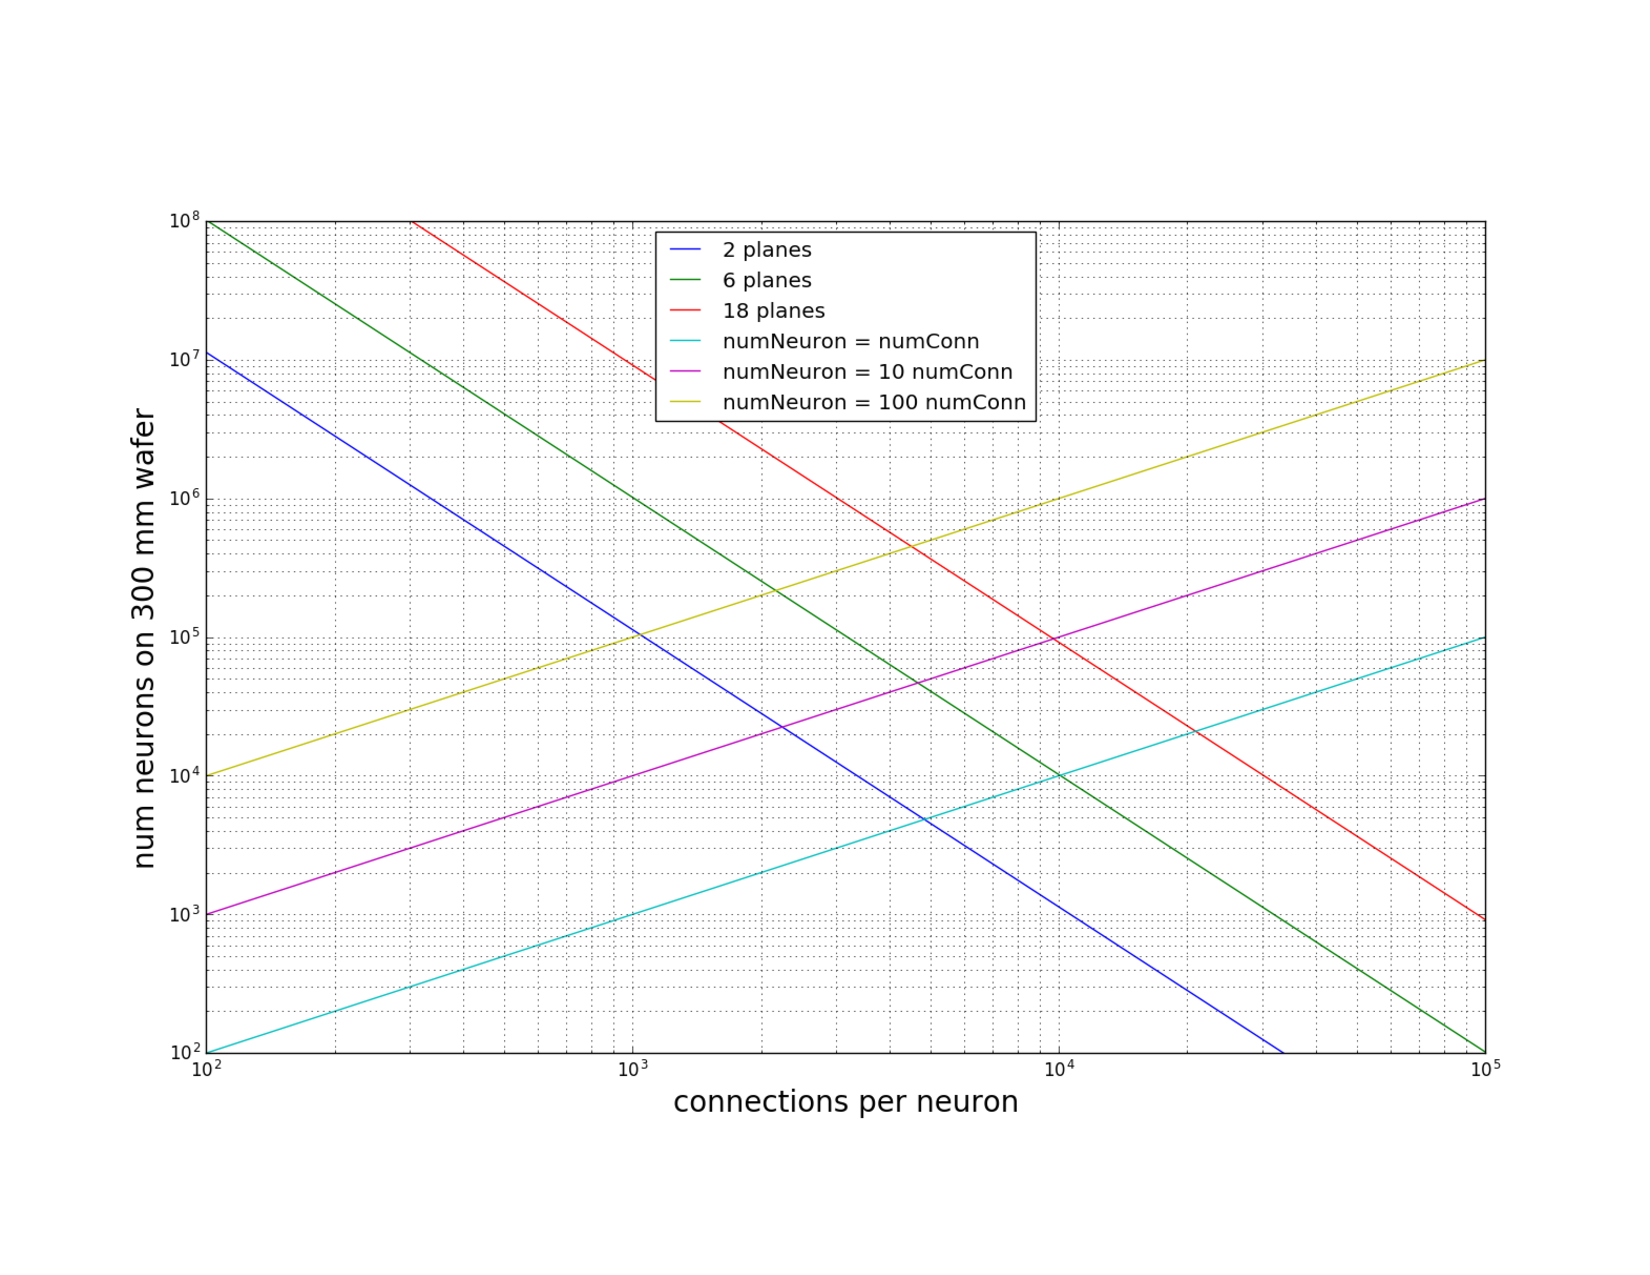
\includegraphics[width=8.6cm]{neuronsOnWafer.pdf}}
%	\captionof{figure}{\label{fig:neuronsOnWafer}Number of neurons on a wafer.}
%\end{figure_alt}
%\begin{figure*}[] 
%	\centering{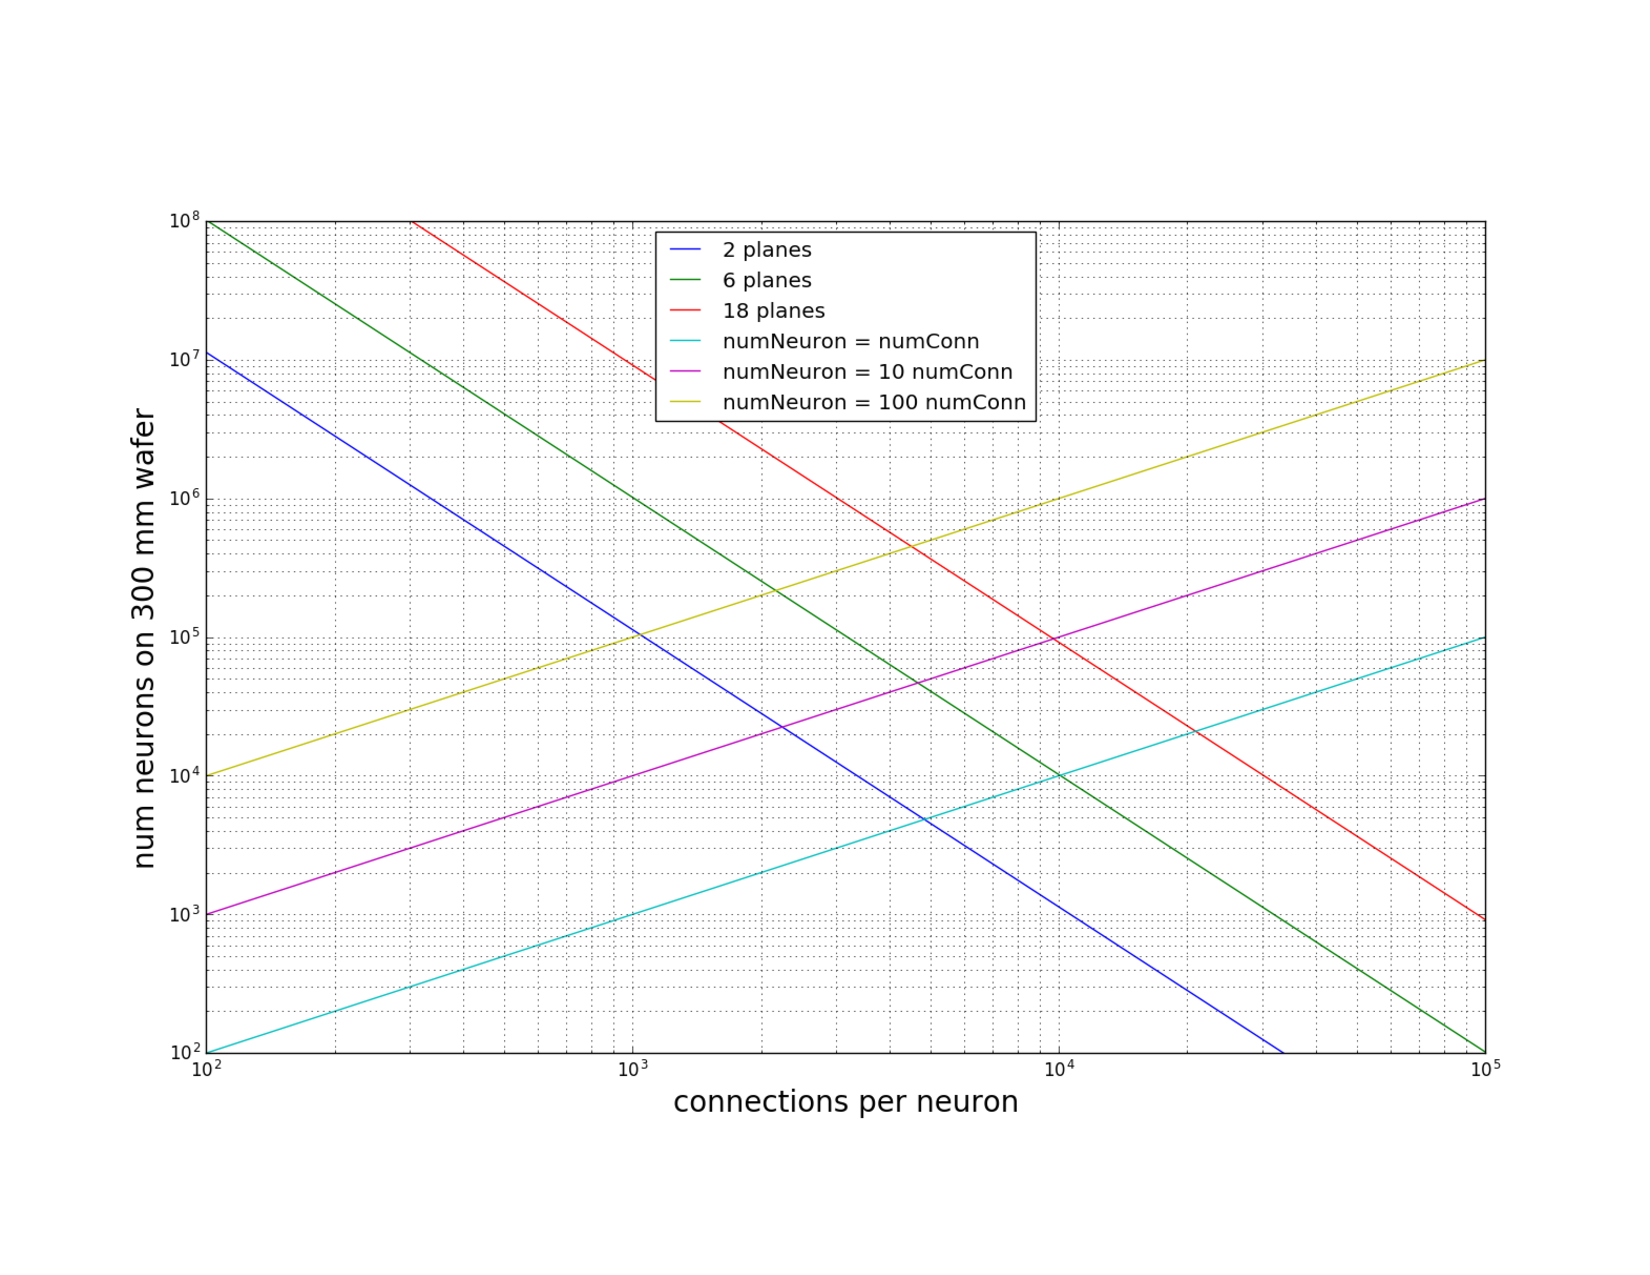
\includegraphics[width=14cm]{neuronsOnWafer.pdf}}
%	\captionof{figure}{\label{fig:neuronsOnWafer}Number of neurons on a wafer.}
%\end{figure*}
This expression is plotted in Fig.\,\ref{fig:neuronsOnWafer}. This estimate informs us that a 300-mm wafer with six waveguide planes can support roughly one million neurons if they each have one thousand connections. As a point of comparison, Ref.\,\cite{kuwa2017} finds that through multi-layer, wafer-scale integration of logic and memory, 250 million electrical neurons could fit on a 300-mm wafer. The trade-off is, of course, speed, as the shared communication network would limit the electrical neurons studied in Ref.\,\ref{kuwa2017} to 10\,Hz operation. Nevertheless, the message of Fig.\,\ref{fig:neuronsOnWafer} is that photonic routing results in large area consumption. If two planes of routing waveguides are used, 100,000 neurons with 1000 connections each can fit on a wafer. With six planes, one million such neurons can fit on a wafer, and with 18 routing planes, the number is close to 10 million. The human cortex contains over 10 billion neurons. An optoelectronic brain larger than a bumble bee will not fit on a wafer.

%\begin{figure*}[] 
%	\centering{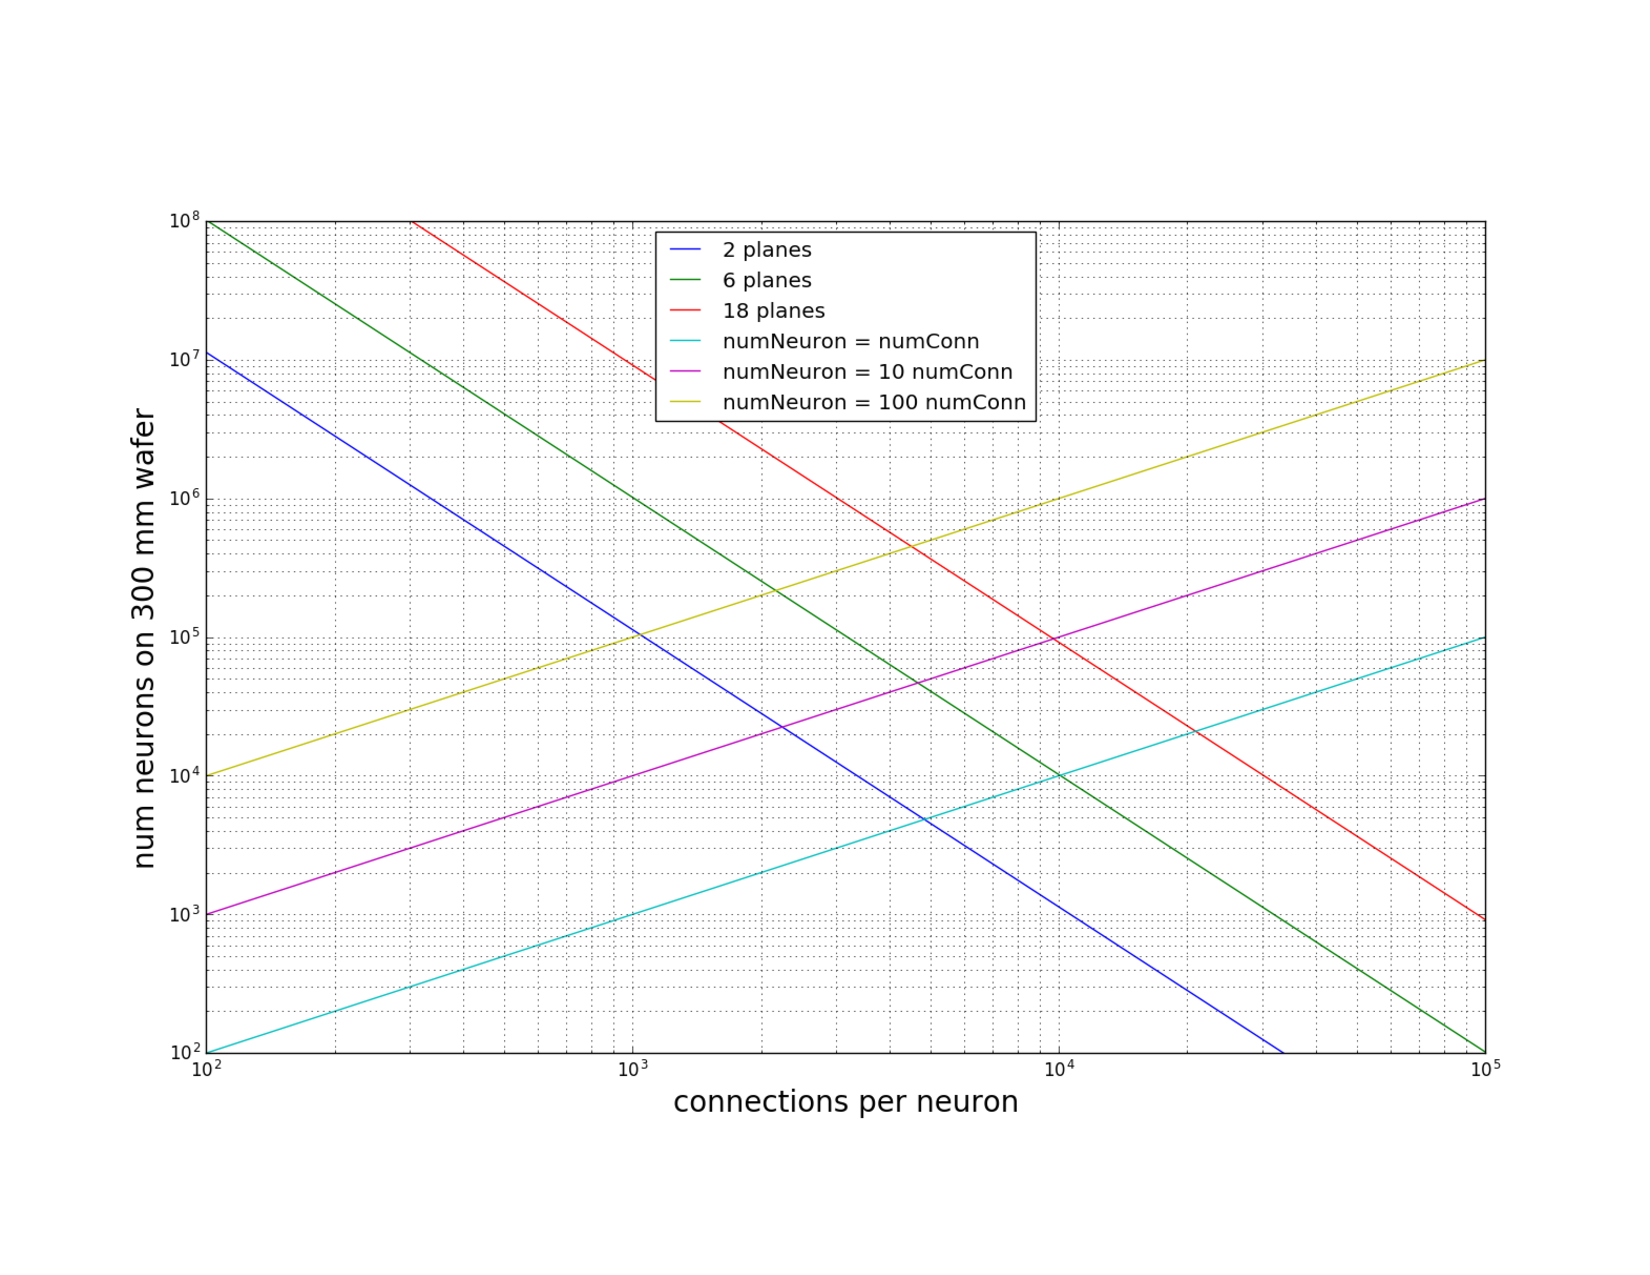
\includegraphics[width=14cm]{communicationScales.pdf}}
%	\captionof{figure}{\label{fig:communicationScales}Photonic interconnection on various length scales.}
%\end{figure*}
Optoelectronic intelligence will require communication between wafers. Wafers can be stacked vertically, and free-space optical links can send photons from a source on one wafer to a detector on a wafer above or below, as illustrated in Fig.\,\ref{fig:communicationScales}(a). Such 3D wafer-stacking techniques are being developed for electronics, but the ability of light to propagate through free space (or liquid helium) and the ten-micron alignment tolerances enabled by wide-area photodetectors \cite{mave2013} make such 3D integration promising for photonic communication as well. Assuming SNSPDs receiving vertical communication have a pitch of 25\,\textmu m, a 300-mm octagon could support $10^8$ vertical communication links between two wafers. Assuming half of this area is for feed-forward communication from the lower wafer to the upper wafer, and half is for feed-back from the upper wafer to the lower wafer. This would result in $5\times10^7$ synaptic connections originating from neurons on one wafer and terminating in neurons on a vertically adjacent wafer. If each wafer had one million neurons with one thousand connections per neuron within the wafer, the total number of intra-wafer synaptic connections would be $10^9$. Therefore, the number of synapses present in a layer of this network that originated on a previous layer would be 5\%, similar to the fraction observed in the laminar structure of biological cortex (Ref.\,\cite{bu2006}, pg. xx).

In addition to free-space vertical coupling, inter-wafer communication can be achieved at wafer edges with in-plane waveguide couplers, as shown in Fig.\,\ref{fig:communicationScales}(c). In the octagonal (truncated square) tiling used here for illustration, each wafer makes such connections to neighbors in the cardinal directions. With a 10\,\textmu m pitch, 11,500 wafer-edge couplers could be supported in each of the cardinal directions with 46,000 total in-plane, lateral connections. Such a system would demonstrate strong connectivity within the vertical stack of the wafers, and weaker lateral connectivity between wafers in the same horizontal plane. Such an architecture resembles the columnar organization of cortex.  

The wafer tiling we have just described leads to a picture of optoelectronic networks with vertically stacked columns of wafers with horizontal connectivity emanating from the perimeter of each wafer. To achieve communication from within these columns to other (perhaps distant) regions of the network, optical fibers are ideal. Within the truncated square tiling under consideration, the square areas at diagonals between wafers can support fiber-optic bundles. These optical fiber tracts are analogous to white matter in the brain. One such region could house a million standard single-mode fibers of 125\,\textmu m diameter. These fibers will emanate from all wafers within the column, so the number of outputs available to each wafer will depend on how many vertically integrated wafers are utilized in a column. If six wafers are stacked in a column, each wafer would have roughly 167,000 output fibers to carry information to distant regions of the network. With one million neurons on a wafer, this would mean not every neuron on the wafer would be able to couple to a fiber for long-distance communication. This again is consistent with brain organization wherein the number of long-distance axons emanating from a region is smaller than the number of neurons within the region. Note, however, that each of these fibers can branch as it propagates through the white matter, so a neuron with access to a single wafer-edge fiber could establish multiple long-range synaptic connections. 
  
%\subsection{\label{sec:scalingToLargeSystems}Scaling to large systems}
%The analogies with biological neural systems has been emphasized: densely connected neurons on wafers can be arranged in columns, comprising the grey matter responsible for computation. Optical fibers between wafers comprise the white matter supporting long-range communication. Notice that we have arrived at this construction based on no specific assumptions about the operation of optoelectronic neurons. We expect the intra- and inter-wafer architecture of optoelectronic neural systems to evolve toward a system like that illustrated in Fig.\,\ref{fig:communicationScales} based solely on the practical considerations of routing light from many sources to many destinations under the constraints of waveguide materials and wafer-scale fabrication. This analysis, while qualitative, elucidates the inevitability of discontinuities in Rentian scaling at certain boundaries. For example, the dense connectivity enabled by high-index dielectric waveguides on a wafer will result in a certain Rent exponent when analyzing only the sub-network contained on a wafer. This exponent may be close to unity, indicating the ability of the network to efficiently integrate information at the wafer scale. However, at the wafer boundary, connectivity is limited, and it will not be possible to maintain the same Rent exponent across partitions of the network containing multiple wafers. Instead, a distinct Rentian analysis is appropriate at this scale wherein it is more suitable to discuss the number of wafers within a partition rather than the number a neurons. A new Rentian exponent will characterize a range of spatial scales from a wafer to perhaps thousands of wafers. Perhaps this Rent exponent will again be close to unity, indicating the ability for each wafer to efficiently communicate with every other wafer within this module. Yet again at some point we will reach a limit, there will be a discontinuity in Rentian scaling, and it will be more appropriate to analyze partitions containing various numbers of these modules, each of which comprises thousands of wafers with millions of neurons per wafer. 

%This modular architecture appears to be inevitable for any computational entity occurring in nature, and it has consequences for how information is processed. The neuroscience community from Mountcastle to the present as well as the VLSI community across similar decades have grappled with the ramifications. Information processing must be simultaneously locally specialized (populations of neurons code for specific stimuli) and globally integrated (network-wide activity affects individual neural behavior). It is the simultaneous local processing of neuronal clusters combined with the global communication amongst neuronal populations that manifests as neuronal avalanches with power-law size distribution. Neuronal avalanches and fractal scaling indicate that increases in network capacity are possible without fundamental reorganization of the system \cite{peth2009}. This form of self-similar information processing has no size limits, in principle. Ultimate limitations will be practical, and related to the inability to maintain continuous Rentian scaling across space and time. The most intelligent system will be the one that can integrate information most effectively across many scales of Rentian hierarchy. It is in this regard that optical communication has the most to offer. On a wafer, photonic fan-out across dielectric waveguides enables neurons to make thousands of direct connections without the limits of a shared switching network. Free-space and wafer-edge couplers enable significant inter-wafer communication conducive to columnar information processing. Such columns can communicate to one another locally and globally over fiber optic links.

On a wafer, photonic fan-out across dielectric waveguides enables neurons to make thousands of direct connections without the limits of a shared switching network. Free-space and wafer-edge couplers enable significant inter-wafer communication conducive to columnar information processing. Such columns can communicate to one another locally and globally over fiber optic links. With this configuration in mind, we can assess the feasibility of constructing systems on the scale of the human cerebreal cortex, with 10 billion neurons, each with thousands of synaptic connections. If a wafer holds a million neurons, a brain-scale assembly requires 10,000 wafers and would fit in a volume two meters on a side\textemdash the size of a few server racks in a closet. 

Several aspects of this technology make the challenge likely to succeed. First and foremost, due to photonic signaing, it remains possible to achieve efficient communication across the network for systems with orders of magnitude more than 10,000 wafers. Information integration across very large neural systems is physically possible with photonic communication. It also appears practically possible, because all the proposed circuits (for loop neurons and perhaps otherwise) can be fabricated at the wafer scale with existing infrastructure (300\,mm silicon-on-insulator substrates, 193\,nm immersion lithography, equivalent of 45\,nm CMOS node). Ten thousand wafers move through a 45\,nm CMOS foundry every day. If such a foundry were dedicated to fabrication of optoelectronic intelligence, it may be able to produce multiple brain-scale systems per year. Assembly of the wafers into a functional system would be difficult, but probably not more difficult than the construction of a contemporary supercomputer. The requirement of liquid-helium cooling is not a major impediment. The greatest unknown is the light source. If silicon light sources that have already been demonstrated in cryogenic optical links \cite{buch2017} can be produced with internal quantum efficiency $\eta_{\mathrm{qe}}\approx 10^{-3}$, we anticipate this project will be economically viable. At present, $\eta_{\mathrm{qe}} = 5\times10^{-7}$ has been demonstrated in the first attempt with no optimization of optical or electrical properties. These light sources need not achieve high performance. We only require they produce incoherent pulses of 10,000 photons ($\approx 1$\,fJ) at 20\,MHz. If no silicon light source operating at 4\,K can meet these criteria, and integration of III-V light sources on silicon wafers is required, the cost and complexity of a project at this scale may become prohibitive.

\section{\label{sec:discussion}Discussion}
At present, the challenge of creating an artificial intelligence rivaling a human appears formidable with the use of silicon electronics alone. The primary challenge arises because direct signaling between large numbers of neurons is not possible due to the charging requirements of wires and devices, so shared communication infrastructure is required, resulting in a connectivity/speed tradeoff. The use of photonic communication will mitigate this tradeoff, despite the increased size of photonic interconnection networks. Photonic fanout enables direct connections between large numbers of neurons, and the velocity of light enables communication across ten-meter systems before communication limits network speed. 

Light is excellent for communication, while electronics excel at computation. Artificial neural hardware should be designed and constructed to maximally leverage photonic communication while performing synaptic, dendritic, and neuronal functions with electronic circuits for complexity of computation. Superconducting optoelectronic circuits appear to naturally implement these functions, in part because light sources and detectors work much better at low temperature, and in part because of the utility of Josephson nonlinearities for neural computation. The von Neumann architecture emerged to perform arithmetic calculations in a manner based on a Turing machine. Neural information processing departs markedly from the sequential operation of a Turing apparatus, so we should not be surprised that optimal hardware may differ. Yet for the superconducting optoelectronic hardware discussed here, the fabrication infrastructure is largely the same as contemporary CMOS. The construction, facilities, and cost of a brain-scale optoelectronic system are likely comparable to a contemporary supercomputer. Understanding the principles of network information processing and designing the architecture to achieve general intelligence are the true grand challenges.

So what are the next steps to realize this technology? Low-cost source-detector integration at the wafer scale is required. These active devices must be augmented with improvements in deposited dielectrics photonic routing enabling more planes with lower loss. For system scaling, improved fiber-to-waveguide coupling and multi-wafer modules must be demonstrated. All the hardware improvements will not lead to AGI without further theoretical analysis at the device, circuit, and system levels. As is the case with other artificial neural systems, theoretical analysis is required to understand how to use these systems, train them, and make them intelligent.

%Amdahl's law draws our attention to the general principle that we should not try too hard to optimize one aspect of a system if performance will only be limited by another aspect. One is hyper aware of this principle when contemplating new hardware for neural systems, precisely because neural systems have intricacies that are interdependent across many functions and scales. Synapses must be designed with a variety of plasticity mechanisms in mind, while simultaneously ensuring nonlinear processing in dendrites and neurons. Computation must be considered alongside communication, and information integration across space must be considered simultaneously with information integration over time. A specific device or mechanism may appear suitable to perform a given function when that function is considered in isolation, but to be successful in cognitive computing, each component must perform well in isolation and integrate well with the rest of the computational hierarchy. Speed matters, but it must be considered in the context of information propagation across the network. Extremely fast oscillators do not bring their full advantage if they cannot communicate effectively to large numbers of other oscillators or if they cannot retain information regarding the history of their inputs. Power consumption is significant, but one may be willing to burn more if performance can be substantially increased, provided the network can be adequately cooled. Size is important, but it must be compared to the distance signals can travel in the period of a network-wide oscillation cycle. The two attributes we find most fundamental are that neural systems require excellent communication, and neural devices require complex computation. Together, these requirements inform our perspective that advanced neural hardware requires optoelectronic integration.

%\vspace{10em}
%Notes:
%\vspace{4em}
%\vspace{4em}
%Must explain: level of devices $\longrightarrow$ synaptic, dendritic, neuronal functionalities for enabling diverse dynamical states, extracting maximal information from spike trains, and efficient retrieval and storage of memories.
%
%network level $\longrightarrow$ neuronal avalanches integrate information across space and time and rely on fractal scaling. for large-scale systems, this means fractal scaling must be supported across spatial and temporal scales. This requires efficient communication without activity-related bottlenecks or connectivity/speed tradeoffs. In the spatial domain, this is enabled by networks that maintain small-world architecture locall as well as globally. In the temporal domain, this is enabled by direct, point-to-point communication unburdened by a shared switching infrastructure. Neuron A must be able to spike and communicate to all of its connections at any time and at any frequency up to its device-limited maximum relaxation oscillation frequency, irrespective of the activity of any other Neuron B in the network.
%
%Scale-free network activity is only possible from the smallest to largest scales (in space and  time) allowed by hardware. It is our perspective that this range can be maximized if electronic and photonic physics are both utilized.
%
%\begin{itemize}
%\item general principles apply to any integrated photonic neural technology
%\item intra-wafer
%
%\begin{itemize}
%\item dense routing on a chip or wafer is best accomplished with high-index-contrast dielectric waveguides
%\item massive connectivity requires multiple planes of dielectric waveguides
%\item index contrast can be generally lowered for larger reach connections with SiNO
%\end{itemize}
%
%\item inter-wafer
%\begin{itemize}
%\item wafer-scale fabrication will place a limit on the number of neurons that can be monolithically integrated. 
%\item inter-wafer communication must be possible. 
%\item free-space: beam divergence?
%\item fiber optic white matter
%\end{itemize}
%
%\item ultimate limits
%\begin{itemize}
%\item at largest scale, all cognitive systems must be limited by the distance light can travel during a network oscillation at a given frequency
%\item speed of light limits what can be thought in our universe
%\item rentian scaling from die-sized neuronal clusters to planet-sized cognitive systems
%\item most significant weakness of photonic systems is size, but ultimately more than compensated by the speed of light
%\end{itemize}
%
%\end{itemize}
%
%\vspace{4em}
%
%\begin{itemize}
%
%\item further comparison to biology
%\begin{itemize}
%\item constituents of brain matter vs artificial (glial cells/silicon matrix, dendritic arbor/superconducting circuitry, axonal arbor/waveguide interconnects, spiking neurons/pulsing light sources, neuromodulators/control currents, water/He)
%\item contrast axon scaling, delay with photonic system
%\item complexity across spatial and temporal scales
%\item system-wide design co-optimization
%\end{itemize}
%
%\item what's next for photonic neural circuits
%\begin{itemize}
%\item similar to what is needed for optoelectronic integration for digital logic
%\item low-cost source-detector integration at the wafer scale
%\item improvements in BEOL photonic routing
%\item demonstration of photonic neural systems beyond a single variable attenuator or relaxation oscillator (Princeton leads the way)
%\item improved fiber-to-chip coupling and multi-chip/wafer modules
%\item scaling up: wafer-scale integration and beyond
%\item further theoretical analysis at device, circuit, and system levels
%\item similar to other artificial neural systems, need theoretical analysis to understand how to use these systems, train them, make them intelligent
%\item AGI requires significant hardware improvements, but hardware alone will not be smart. that requires insight from device to architecture, neuron to network, across space and time.
%\end{itemize}
%
%
%\end{itemize}
%
%\vspace{4em}
%There are $10^{14}$ synapses in the human cortex. If it takes even 10\,nW to maintain the state of each synapse, the system will consume a megawatt just to remember what it has learned. This is one reason superconducting synapses are attractive: they can maintain a memory indefinitely with no static power dissipation. Additionally, the strength of a synapse can be increased or decreased based on single-photon detection events. STDP appears possible with a single photon for each step of the update process. 
%
%\vspace{4em}
%Suppose we could get around fabrication considerations and construct arbitrary neural systems based on biological neurons. Would we then choose to pursue that technology for beyond-human intelligence instead of developing optoelectronic hardware? We think not, because the slow conduction velocity of axons presents a limit to communication, and this limit is likely already saturated near the scale of the human brain. If this argument is correct, we should not expect genetic engineering to achieve much smarter people than have already walked the earth.

%\begin{equation}
%P(s) = cs^{-\alpha}
%\end{equation}
%
%\begin{equation}
%e = cn^{-p}
%\end{equation}
%
%\begin{equation}
%d = \frac{1}{1-p}
%\end{equation}

%\bibliographystyle{abbrv}	
\bibliography{light_in_neural_systems}

%\end{multicols}

\end{document}